% Chapter 3 - APIs, enlace con las modalidades

\chapter{Enlace con las modalidades} % Chapter title

\label{ch:enlace} 

%----------------------------------------------------------------------------------------

% ### Introducción de capítulo

 
\section{Arquitectura Propuesta} \label{sec:enlace_overview}
%Primer vistazo general de los ''endpoints'' del sistema, que conectamos? como se consume?
A grandes rasgos, los puntos de entrada a la plataforma \emph{Plusultra} introducida en el capítulo anterior, estarán ubicados en dos lugares diferentes:

\begin{itemize}
\item \textbf{Clientes Web}; aquí también reside la lógica de la aplicación. En conjunto crean una experiencia multimodal en la web. Dentro de los clientes web, podemos encontrar capacidades extra que pueden ser usadas a su vez como modalidades (\ie ~un cliente corriendo en un smartphone puede tener acceso a sensores, que a su vez, pueden ser usados como reconocedores). Mas adelante en este capítulo, se analizará esta situación.
\item \textbf{Dispositivos de modalidad}; se refiere a todos aquellos dispositivos especialmente dedicados a reconocer o sintetizar una modalidad, \eg~ Falcon de Novint o Leap Motion, por mencionar algunos.
\end{itemize}

Para conectar estos puntos de entrada, se construyo un modulo de acceso que puede ser consumido por igual tanto del lado del cliente como del servidor o \emph{standalone} (dispositivos de modalidad). Ademas se ha desarrollado una primera versión de un protocolo de comunicación que acompaña dicha interfaz de comunicación. Este protocolo abre el camino a otros desarrolladores para que puedan diseñar soluciones utilizando diferentes lenguajes. 
En el mismo se describe los mensajes utilizados para un enlace efectivo con la plataforma \emph{Plusultra}. De esta manera, siguiendo a este protocolo versionado, la API puede portarse a otros lenguajes de programación extendiendo así el alcance y uso de la plataforma.

\subsection{Modulo Híbrido Cliente/Servidor}
Prácticamente todo el desarrollo de este trabajo se ha llevado a cabo utilizando el lenguaje JavaScript. Dado que se busca expandir la capacidad actual de comunicación de las aplicaciones web, es lógico basar la mayor parte de la base de código en dicho lenguaje. Usando la plataforma Node.js, es posible correr JavaScript del lado del servidor también, haciéndolo ubicuo en múltiples escenarios. Teniendo en cuenta estas capacidades, se decidió desarrollar un modulo que pueda aprovechar estos aspectos y ser de utilidad en diversas circunstancias o casos de uso.
 
De esta forma se introduce el módulo \emph{Gyes}. A través de este componente es posible conectarse al sistema, transmitir datos de modalidades, crear nuevas modalidades, crear interpretaciones, capturar salidas del sistema de fisión; por nombrar los casos mas importantes. 

\subsection{Vista General}
%Grafico que muestre los componentes introducidos antes y las nuevas interfaces.
El modulo \emph{Gyes} permite realizar diferentes tareas, las cuales tienen como finalidad interactuar con la plataforma \emph{Plusultra} y por consiguiente con el resto de los actores de la aplicación, es decir, con el contexto entero de la aplicación web.
El siguiente gráfico \ref{fig:arq_ours_gyes_action} simplifica una de las principales actividades, utilizar una modalidad como reconocedora de algún tipo de señal para luego propagarla en la aplicación, mediante la plataforma. 

% FIGURA DE GYES en accion
\begin{center}
  \begin{figure}[h]
    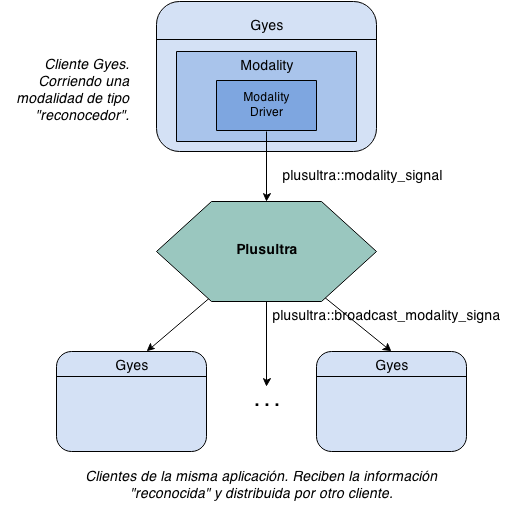
\includegraphics[scale=0.7]{gfx/gyes_action}
    \caption{Modulo Gyes en acción: transmitiendo señales}
    \label{fig:arq_ours_gyes_action}
  \end{figure}
\end{center}

\section{Descripción de la Interfaz del Modulo} \label{sec:enlace_api}
% detalles de la interfaz
En la figura \ref{fig:arq_ours_gyes} se observa de manera directa los principales componentes del modulo de acceso al sistema. Luego extenderemos esta visión a la interacción que ocurre con la plataforma.
A continuación se describirán las interfaces de los componentes junto a una breve introducción a la primer version del protocolo de comunicación entre \emph{Plusultra} y \emph{Gyes}.

% FIGURA DE COMPONENTES GYES
\begin{center}
  \begin{figure}[h]
    \centering
    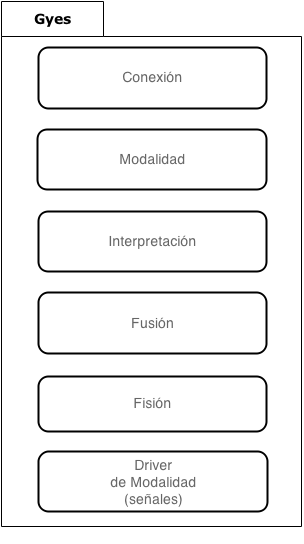
\includegraphics[scale=0.7]{gfx/gyes}
    \caption{Principales componentes del modulo Gyes}
    \label{fig:arq_ours_gyes}
  \end{figure}
\end{center}

\subsection{Componente de Conexión}

Es el componente principal. Desde aquí no solo accedemos a la plataforma si no también al resto de los componentes. 

La función principal es proveer una forma de conectar, tanto para modalidades como clientes a \emph{Plusultra}.
\\

\underline{\textsf{Constructor:}}\\
\begin{lstlisting}
Gyes( appKey, uri, opts )
\end{lstlisting}
Crea una nueva instancia del módulo \emph{Gyes}. Automáticamente inicia una conexión con la plataforma \emph{Plusultra}.
\\ 

\underline{\textsf{Principales métodos:}}\\
\begin{itemize}
\item[]
\begin{lstlisting}
gyes::authenticate( appKey )
\end{lstlisting}
Una vez creada la instancia, necesitamos autenticar nuestra aplicación. Para eso el desarrollador web debe contar con una llave, previamente generada, por ejemplo usando algún servicio donde registre la aplicación y la cantidad de instancias a consumir de la plataforma.
\\

\emph{Plusultra} es una plataforma que ha sido diseñada para ser fácilmente escalable a un modelo de PAAS (\emph{Platform as a Service}), de esta forma, múltiples instancias del módulo de plataforma pueden servir a diferentes aplicaciones. Por eso es necesario que cada aplicación posea una llave que la distinga.

\item[]
\begin{lstlisting}
gyes::addModality( aModality )
\end{lstlisting}
Permite agregar una nueva modalidad al sistema. Esto es útil para indicar que determinado cliente cuenta con una modalidad particular la cual, al estar ``agregada'' a la plataforma, puede compartir la información que genera.
\end{itemize}

\subsection{Componente de Modalidad}
%diagrama de secuencia, conexion, fusion/fision

Este módulo permite crear y agregar nuevas modalidades al sistema. Dada la naturaleza variada de las mismas, se decidió separar comportamiento de representación/identificación. El comportamiento esta definido por los drivers, aquí especificamos una representación. Dentro de una aplicación, pueden conectarse mas de una modalidad y por ahora, una modalidad puede usar un driver.
\\

\underline{\textsf{Constructor:}}\\
\begin{lstlisting}
Gyes::Modality( name, type, opts )
\end{lstlisting}
Permite crear un nuevo objeto que representa a una modalidad, la cual podrá ser agregada al sistema. Recibe un nombre (\emph{name}), tipo (\emph{type}), de acuerdo a si es de entrada/salida o ambos y luego opciones (\emph{opts}) particulares para compatibilidad a futuro.
\\

\underline{\textsf{Principales Métodos:}}\\
\begin{itemize}
\item[]
\begin{lstlisting}
modality::use( modalityDriver )
\end{lstlisting}
Conecta una instancia de modalidad con una instancia de driver.
\end{itemize}

\subsection{Componente de Fusión Distribuida}

Permite controlar el motor de fusión de manera programable. Este componente captura \emph{señales} que pueden ser generadas por modalidades o por eventos de la aplicación.
\\

\underline{\textsf{Constructor:}}\\
\begin{lstlisting}
Gyes::Fusion( opts )
\end{lstlisting}
Genera una nueva instancia del motor de fusión. 
\\

\underline{\textsf{Principales métodos:}}\\
\begin{itemize}
\item[]
\begin{lstlisting}
fusion::fuse( anInterpretation )
\end{lstlisting}
Detecta un determinado conjunto de señales, definidos por una interpretación. Cuando dicha interpretación ocurre, puede distribuir esta información entre todos los clientes y comenzar el proceso de activar al sistema de fisión.
\\

La captura de señales se produce manteniendo una ventana de tiempo, donde la misma se actualiza (extiende) cada vez que ocurre un evento que pertenezca a una interpretación. Esto ocurre de forma independiente y distribuida entre todos de la aplicación. Es decir, cada uno cuenta con un motor de fusión. Para que esto funcione, las señales deben ser distribuidas, usando la plataforma, en tiempo real.
\end{itemize}

\subsection{Componente de Fisión Distribuida}

Brinda acceso al sistema de fisión. El desarrollador web, encuentra en este componente un ``punto de salida'' de la plataforma, donde puede conectar la lógica de la aplicación web mientras consume información generada por las distintas señales que recorren el sistema.
\\

\underline{\textsf{Constructor:}}\\
\begin{lstlisting}
Gyes::Fission( opts )
\end{lstlisting}
Genera una nueva instancia del motor de fisión.
\\

\underline{\textsf{Principales Métodos:}}\\
\begin{itemize}
\item[]
\begin{lstlisting}
fission::on( interpretationName, callbackFn )
\end{lstlisting}
El sistema de fisión permite al desarrollador conectar la ocurrencia, asincrónica, de una interpretación con código que afecte a la lógica de negocios de la aplicación.
\end{itemize}

\subsection{Componente de Interpretación}

En los componentes anteriores se menciono el concepto de \emph{interpretación}, aquí se muestra su interfaz y lo que representa.

Este componente permite agrupar un conjunto determinado de señales en un único objeto.
Una interpretación puede representar la conjunción de diferentes modalidades en un único evento.
Las interpretaciones son usadas por el motor de fusión para detectar la ocurrencia de dichas señales e interpretarlas como un único evento alertando al resto de los componentes del sistema sobre dicha ocurrencia.
\\

\underline{\textsf{Constructor:}}
\begin{lstlisting}
Gyes::Interpretation( eventsList )
\end{lstlisting}
Genera una nueva instancia de interpretación. Recibe una lista de señales la cual servirá para organizar al sistema de fusión en el escaneo y detección de ocurrencias de interpretaciones.
\\

\underline{\textsf{Principales Métodos:}}\\
\begin{itemize}
\item[]
\begin{lstlisting}
interpretation::getName()
\end{lstlisting}
Regresa una identificación única para la interpretación. Útil para ``escuchar'' por una determinada ocurrencia.

\item[]
\begin{lstlisting}
interpretation::canSynthetize( modalityID,modalityDriverID,param )
\end{lstlisting}
Permite activar desde la lógica de la aplicación alguna capacidad de sintetizado provista por algún driver de modalidad. Recibe un identificador de modalidad (\emph{modalityID}), un identificador de driver de modalidad (\emph{modalityDriverID}) y parámetros (\emph{params}) opcionales para la función de sintetizado.

\end{itemize}

\subsection{Componente de Driver de Modalidad}

Brinda una interfaz para el desarrollo de diferentes comportamientos sobre una modalidad. Esto permite que la plataforma sea agnóstica a una determinada modalidad particular. A través del uso de señales, el desarrollador de driver de modalidad, podrá escribir la lógica necesaria para su dispositivo de modalidad, ya sea un \emph{reconocedor}, \emph{sintetizador} o de ambos tipos; y conectar esa lógica de forma uniforme a la plataforma.
\\

\underline{\textsf{Constructor:}}\\
\begin{lstlisting}
Gyes::ModalityDriver()
\end{lstlisting}
Genera una instancia que contiene las diferentes señales para conectarse con el cliente y así con la plataforma.
\\

\underline{\textsf{Principales Métodos:}}\\
\begin{itemize}
\item[]
\begin{lstlisting}
modalityDriver::on( signal, callbackFn )
\end{lstlisting}
Permite al desarrollador de driver de modalidad, conectar de forma clara una señal de sintetizado (\emph{synthetized}) o actualización (\emph{updated}) con funcionalidad propia del driver.
\item[]
\begin{lstlisting}
modalityDriver::fire( signal, data )
\end{lstlisting}
Permite disparar una señal de reconocimiento (\emph{recognized}), acompañado de datos producidos por la modalidad. Esta información sera distribuida mediante la plataforma.
\end{itemize}

\subsection{Descripción del Protocolo} \label{subsection:protocol}
Se definió un protocolo de comunicación entre la plataforma y los múltiples clientes \emph{Gyes}. El mismo permite expresar los conceptos definidos durante el trabajo. Estos son: modalidades, señales e interpretaciones. Se utilizo la notación JSON para definirlo.

A través del uso del protocolo podrían crearse clientes en otros lenguajes, que serian capaces de interactuar de igual forma con la plataforma que el cliente Gyes aquí propuesto (desarrollado en JavaScript). 

A continuación se detallan los eventos que conforman el protocolo en la versión 1.

\begin{center}
    \begin{tabular}{| l | l |}
    \hline
    ID & PARÁMETROS:TIPO \\ \hline
    plusultra::authenticate & appKey:string \\ \hline
    plusultra::welcome & - - - \\ \hline
    plusultra::new\_modality & modality:object \\ \hline
    plusultra::broadcast\_new\_modality & modality:object\\ \hline
    plusultra::modality\_signal & signal:object \\ \hline
    plusultra::broadcast\_modality\_signal & signal:object \\ \hline
    plusultra::interpretation & interpretation:object \\ \hline
    plusultra::broadcast\_interpretation & interpretation:object \\
    \hline
    \end{tabular}
\end{center}

\section{Cuestiones Importantes}
Tener a los módulos de fusión y fisión \emph{distribuidos}, es un acercamiento que plantea desafíos.

En primer lugar, cualquier aplicación distribuida gana mayor poder de computo de forma mucha mas ``económica'' ante una variante centralizada. Luego, la decisión de hacer esta solución \emph{distribuida}, esta relacionada directamente con la arquitectura de bajo nivel del ambiente, es decir, la web. Por lo tanto, el acercamiento \emph{per se} no fue forzado, esto dejo lugar a poder ver claramente como podían desarrollarse los aspectos propios del problema, \ie los diferentes componentes que hacen a una aplicación multimodal. Para ello, se partió de la definición clásica de  \citet{dumas2009multimodal}. 

Allí se identificaron los principales componentes a exportar dentro de esta solución. En particular se descartaron, o no se implementaron directamente, el sistema de administración de dialogo (\emph{Dialog Management}) y el sistema de manejo de contexto/historia del usuario (\emph{Context User Model History}). La decisión se basa en que estos componentes pueden ser mantenidos indirectamente en la lógica de la aplicación web, de acuerdo a la necesidad del desarrollador; además la ausencia de estos componentes de forma directa, facilita la transición hacia un modelo distribuido ya que presentan características de aplicación centralizada, \ie~ no hace necesidad de un servicio externo manteniendo esta información.

De todas formas, se mantiene abierto el análisis, específicamente al componente de administración de dialogo, si se detecta alguna manera concreta en la que pueda mejorar la calidad de uso de la herramienta en general.

Si bien, un sistema multimodal con componentes de fusión y fisión distribuidos, puede generar demasiados mensajes y estos pueden afectar su performance general, la solución propuesta esta diseñada para ser escalable, añadiendo mas instancias de \emph{Plusultra} que a su vez puedan manejar mas volumen de mensajes en el tiempo. 

Uno de los aspectos que inicialmente se agrego como distribuido y luego de algunas pruebas se determino que sea mantenido localmente, fue el componente de modalidad. En un principio, al agregar una modalidad a la plataforma, mediante el cliente \emph{Gyes}, la misma era transmitida a todos los demás clientes web. Esto generaba un problema al momento de disparar una interpretación, ya que la misma podía tener asociada una capacidad de sintetizado y si se intentaba activar dicha capacidad en la modalidad recibida por la plataforma, podría ocurrir un error o en un caso silencioso, un gasto de mensajería en vano.
La clave de la plataforma se encuentra en los mensajes que distribuye, estos son: señales de modalidad e interpretaciones (conjunto de señales agrupadas bajo algún valor lógico). Cualquier otro mensaje a ser distribuido puede añadir valor agregado con un costo que debe ser tenido en cuenta porque añade mas mensajería a una plataforma en tiempo real, lo cual puede repercutir directamente en su performance. 

\section{Resumen del Capítulo} \label{sec:enlace_summary}
En el presente capítulo se termino de introducir a los principales actores de la arquitectura de la solución propuesta. En particular, se han descrito aquí a aquellos relacionados a los puntos de entrada/salida del sistema. Estos componentes, en su mayoría, tienen algún tipo de relación con la lógica de la aplicación web donde sean usados; o con la modalidad que se desee integrar al sistema. 

Particularmente, se ha incluido el módulo multiuso \emph{Gyes}, el cual representa una solución tanto para el browser como \emph{standalone}. También se agrega la primer version del protocolo de comunicación entre el cliente y la plataforma, con el fin de dejar abierta una puerta para el desarrollo de otros clientes en diferentes lenguajes. Finalmente se destacan algunos puntos característicos de esta solución distribuida. Mas investigación en este punto puede ocurrir en el futuro, con el desarrollo de mas y variadas aplicaciones que consuman esta plataforma.